\section{The Compact Muon Solenoid experiment}
\label{cms}
The Compact Muon Solenoid experiment (CMS) is designed for the general study of the highest-energy, highest-luminosity proton-proton (and heavy ion) collisions the LHC can provide. The detector design is driven by the particular goals of exploring physics at the \si{\TeV} scale and discovering the origin of electroweak symmetry breaking \cite{cms_tdr_v2}. More than 4000 collaborators from institutions across more than forty countries work together to collect and analyze the data using a global computing grid \cite{cms_collaboration}.

To reconstruct the variety of particles that emerge from high-energy proton-proton collisions, CMS uses several complimentary subdetectors nested radially about the collision point. A \SI{4}{\tesla} superconducting solenoid magnet provides a powerful magnetic field to bend the trajectories of charged particles, thus enabling the determination of their momenta. Working from the center out, the CMS detector consists of an all-silicon tracker, a lead-tungstate scintillating crystal electromagnetic calorimeter, a sampling hadronic calorimeter composed of brass absorber and plastic scintillator tiles, the superconducting solenoid magnet, and a muon system with three varieties of gaseous detectors. Figure~\ref{cms_detector_cartoon} shows the detector layout, and the remainder of this chapter is devoted to a brief overview of each subsystem as well as the triggering and reconstruction strategies employed by CMS.

\begin{figure}
\centering
\includegraphics[width=0.8\textwidth]{figures/lhc_and_cms/cms_detector_cartoon.pdf}
\caption{The CMS detector~\cite{cms_detector_cartoon}.}
\label{cms_detector_cartoon}
\end{figure}

CMS uses a right-handed coordinate system centered on the nominal collision point with positive $x$ direction pointing towards the center of the LHC ring and the positive $y$ direction pointing vertically upward. The azimuthal angle in the $x$-$y$ plane, denoted $\phi$, is measured from the positive $x$ axis, and the polar angle $\theta$ is measured from the positive $z$ axis. The angle from the $z$ axis is more commonly described in terms of the pseudorapidity $\eta=-\ln\tan(\theta/2)$. Distances in the $\eta$-$\phi$ plane are commonly referred to as $\Delta R = \sqrt{(\Delta \eta)^2 + (\Delta \phi)^2}$. The component of the momentum that is transverse to the beam direction (i.e., in the $x$-$y$ plane) is denoted \pt, and the magnitude of the negative vector sum of the \pt of all the reconstructed particles in an event is denoted \ptmiss \cite{cms_tdr_v1, cms_experiment}. \fxnote{could include a diagram if I want}

The CMS detector has undergone several upgrades since its initial construction. The description presented here will focus on the detector conditions relevant to the analysis presented in Section~\ref{displaced_leptons}.

\subsection{Solenoid magnet}
The superconducting solenoid is designed to produce a \SI{4}{\tesla} magnetic field throughout the \SI{6.3}{\metre} diameter, \SI{12.5}{\metre} long cylindrical volume that contains the tracker and calorimeters. The magnetic field is produced by running \SI{19}{\kA} through 2168 turns of NbTi superconducting cable that are cooled with liquid helium. The flux returns through an iron yoke that also houses the muon system \cite{cms_experiment}.

The strong magnetic field is critical to CMS's ability to unambiguously distinguish muons and anti-muons with transverse momenta up to \SI{1}{\TeV} \cite{cms_tdr_v1}, and much of the overall detector design is guided by the choice of a large superconducting solenoid. The uniform magnetic field alters the trajectories of charged particles immediately upon their production, which results in significant bending power within a relatively small radius and therefore enables a compact detector.

The CMS solenoid stores a uniquely large amount of energy in its magnetic field when compared to other collider detector magnets, especially when viewed relative to its mass. To avoid deformations from the strong magnetic field, the superconducting coils are reinforced with an aluminium alloy so that the coil layers themselves handle 70\% of the magnetic hoop stress. Figure~\ref{solenoid_figures} compares several collider detector magnets in the energy/mass vs energy plane and shows a cross-sectional view of the reinforced conductor coils in cross section. This approach allows for a relatively thin solenoid that is less likely\fxnote{relative to what?} to scatter muons before they reach the muon system \cite{cms_experiment}. 

\begin{figure}
\centering
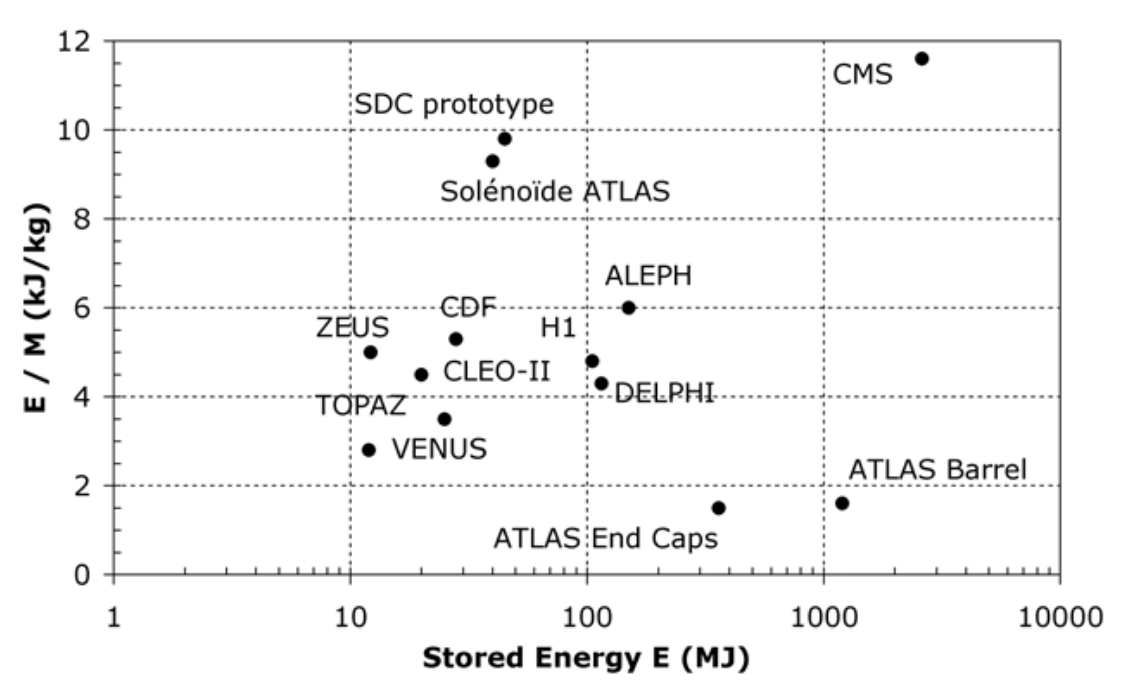
\includegraphics[width=0.65\textwidth]{figures/lhc_and_cms/solenoid_energyOverMass_vs_mass.png}
\hspace{5 mm}
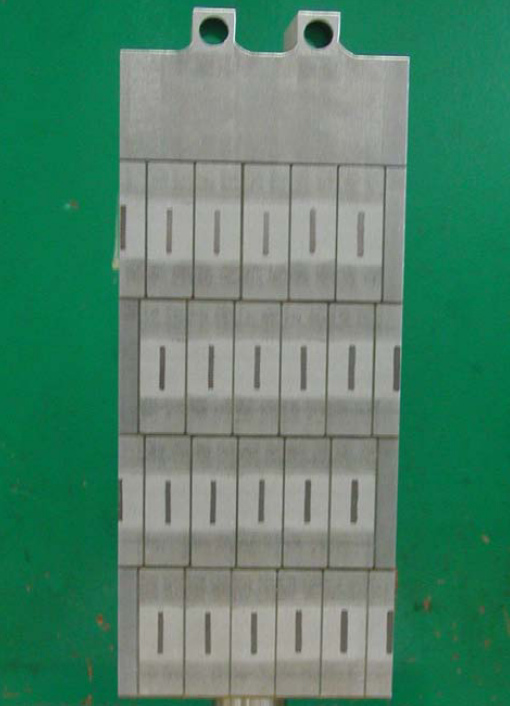
\includegraphics[width=0.28\textwidth]{figures/lhc_and_cms/solenoid_cross_section.png}
\caption{The stored-energy-over-mass ratio, $E/M$, for several detector magnets (left), and a cross-sectional view of the four-layer winding of reinforced conductor in the CMS superconducting solenoid (right)~\cite{cms_experiment}.}
\label{solenoid_figures}
\end{figure}

\subsection{Tracker}
\label{tracker}
In the region closest to the proton collisions, CMS employs a silicon tracker to reconstruct particle trajectories along with primary and secondary vertices. Efficiently and accurately performing these tasks allows CMS to measure charged particle momenta, distinguish between particles from the primary and pileup\fxnote{have I defined pileup?} vertices, and identify heavy-flavor decays. The high particle flux necessitates a highly granular, fast, and radiation hard detector that introduces the smallest possible amount of material to the region inside the calorimeters. The resulting detector contains over \SI{200}{\m\tothe{2}} of active silicon, making it the largest silicon tracker ever built. The tracker has a length of \SI{5.8}{\m}, a diameter of \SI{2.5}{\m}, and is divided into two subdetectors. Inside a radius of \SI{20}{\cm}, the particle flux demands the use of silicon pixel detectors, while silicon micro-strip detectors suffice in the region beyond \SI{20}{\cm} \cite{cms_experiment}. 

The pixel and strip detectors both utilize the same fundamental detection mechanism: the energy depositions of incident charged particles form electron-hole pairs when passing through the depletion region of a reverse-biased p-n\fxnote{note subtlety here?} junction, and the resulting induced current signifies the presence of a charged particle. The reverse bias voltage sweeps away charge carriers to reduce thermal noise and maximize the sensitive volume.\fxnote{mention cooling?} The fine two-dimensional segmentation of the pixel detector provides precise two-dimensional position measurements from a single detector layer, while each strip detector layer only provides a one-dimensional location measurement. In both cases, the detector planes are tilted to allow the charge liberated by a single incident particle to spread across multiple pixels or strips. This scheme significantly improves the position resolution by combining the charge measurements of multiple adjacent pixels or strips.

The original pixel detector was replaced between the 2016 and 2017 data-taking periods in preparation for higher luminosities \cite{cms_phase1_pixels}. As the analysis presented in Section~\ref{displaced_leptons} uses data collected in 2016--2018 and is particularly dependent on tracker measurements, the original pixel detector, 2017--2018 (Phase-1) pixel detector, and strip detector are described separately below.

\subsubsection{Original pixel detector}
The original CMS pixel detector covers the $|\eta|<2.5$ region and is composed of three cylindrical barrel layers at $r=4.4$, $7.3$, and \SI{10.2}{\cm} and four endcap disks \num{34.5} and \SI{46.5}{\cm} up and down the beamline from the nominal collision point. Each layer or disk is instrumented with several pixel modules that are composed of a silicon sensor bump bonded to custom ASIC read-out chips (ROCs). Each sensor is \SI{285}{\um} thick and typically comprises \num{66560} $100\times\SI{150}{\um}$ pixels. The nearly square pixel shape enables approximately \SI{15}{\um} hit resolution in both the $r$-$\phi$ and $z$ directions \cite{cms_tdr_v1, cms_experiment}.

\fxnote{describe sensors and readout}

The original pixel detector was designed for a maximum instantaneous luminosity of \SI{e34}{\cm\tothe{-2}\s\tothe{-1}}, which corresponds to approximately 25 pileup collisions per bunch crossing in CMS. As shown in Fig.~\ref{lhc_lumi}, the LHC first exceeded this instantaneous luminosity in 2016. Figure~\ref{pixel_efficiency_2016} shows the resulting hit efficiency loss in the innermost layer of the pixel detector as a function of instantaneous luminosity and number of pileup collisions per bunch crossing. While the higher-radius pixel layers are less affected, important quantities such as the transverse impact parameter resolution are highly dependent on the measurements of the layer closest to the interaction. To mitigate this effect, CMS replaced the original pixel detector between the 2016 and 2017 data-taking periods. 

\begin{figure}
\centering
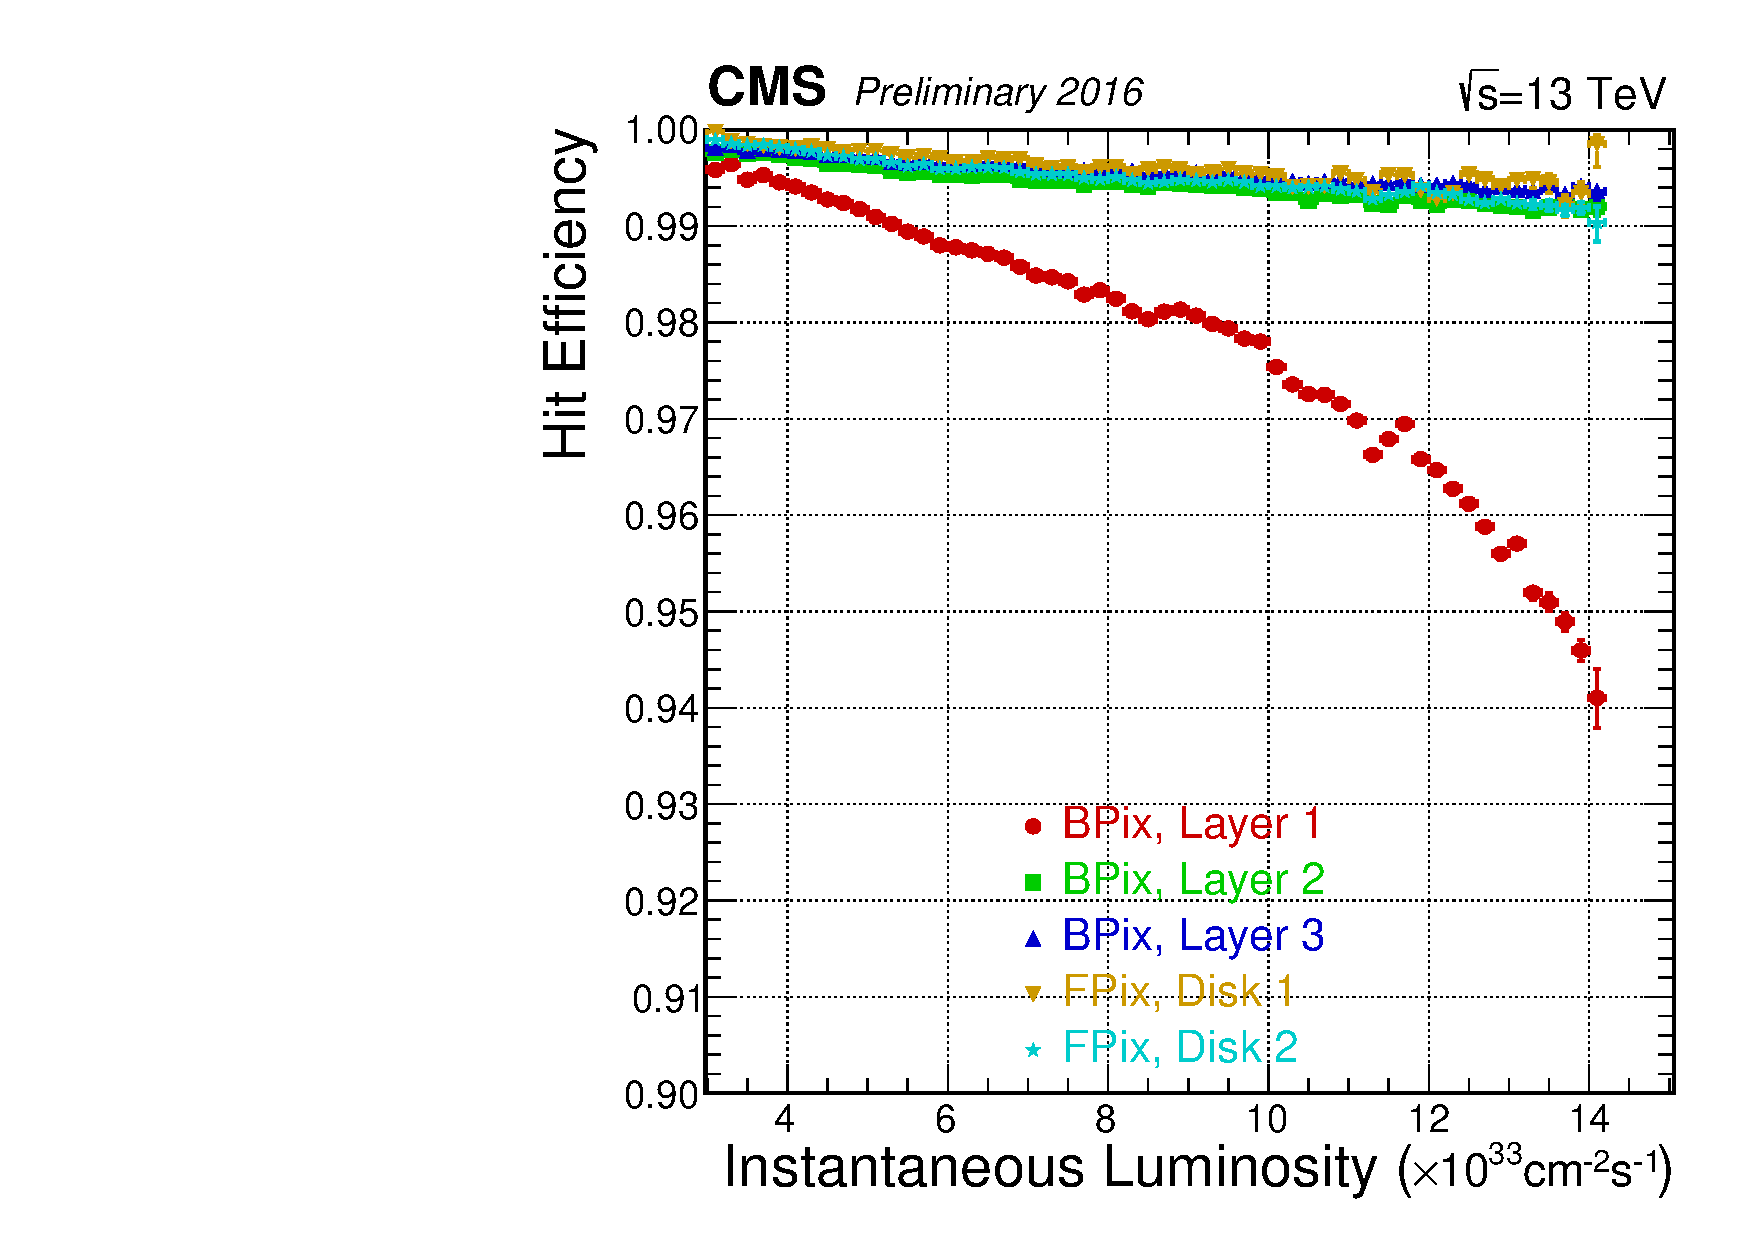
\includegraphics[width=0.45\textwidth]{figures/lhc_and_cms/pixel_efficiency_vs_lumi_2016.pdf}
\hspace{5 mm}
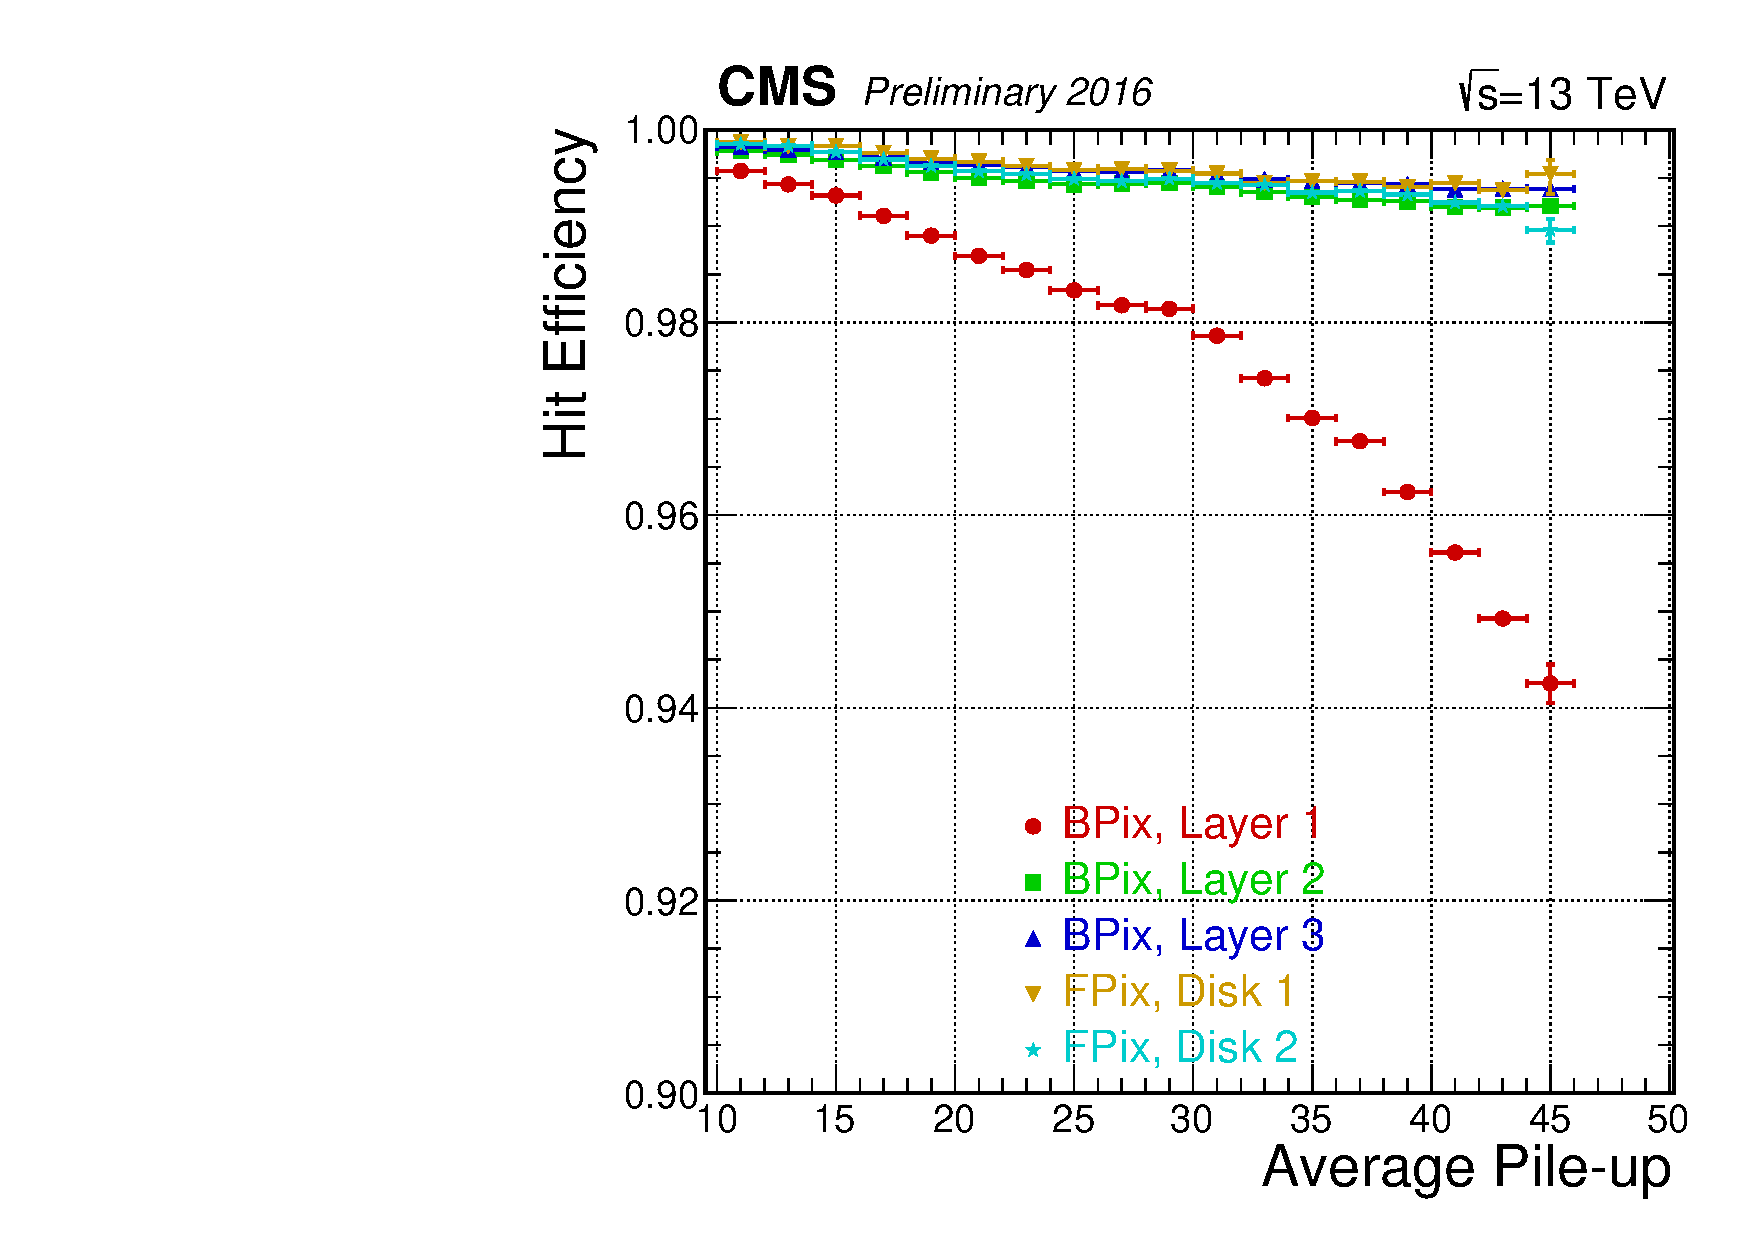
\includegraphics[width=0.45\textwidth]{figures/lhc_and_cms/pixel_efficiency_vs_pu_2016.pdf}
\caption{Measured single hit efficiency per layer as a function of the instantaneous luminosity (left) and inelastic collisions per bunch crossing (right) in data taken with the original CMS pixel detector in 2016 \cite{pixel_performance_plots_2016}.}
\label{pixel_efficiency_2016}
\end{figure}

\subsubsection{Phase-1 pixel detector}
The Phase-1 pixel detector represents an incremental improvement over the original CMS pixel detector: the same fundamental technology fills the same physical footprint and reuses many of the existing services but nevertheless achieves higher rate capabilities, improved radiation tolerance, and more robust tracking \cite{cms_phase1_pixels}. This is achieved by adding one additional layer to the barrel and each endcap, decreasing the radius of the innermost barrel layer to \SI{2.9}{\cm}, upgrading the ROCs, and reducing the material budget of the cooling system and mechanical structure \cite{cms_phase1_pixels, cms_phase1_pixel_tdr}. Figure~\ref{pixels_original_vs_phase1} compares the geometries of the original and Phase-1 pixel detectors.

\begin{figure}
\centering
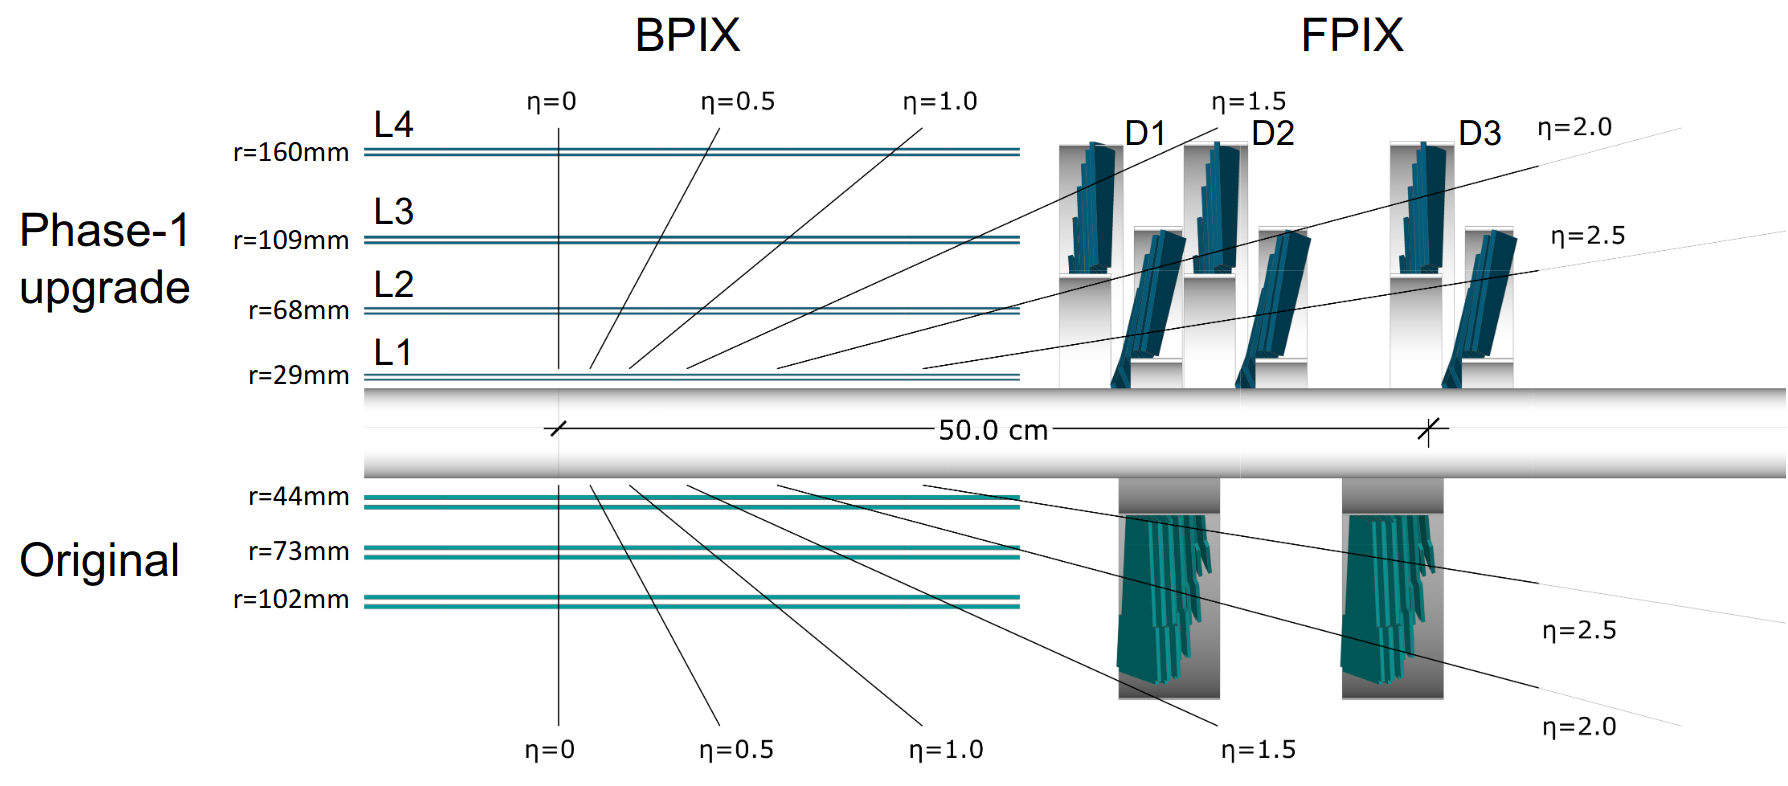
\includegraphics[width=0.9\textwidth]{figures/lhc_and_cms/pixels_layout_comparison.png}
\caption{Comparison of the original and Phase-1 CMS pixel detector layouts in $y$-$z$ plane~\cite{cms_phase1_pixels}.}
\label{pixels_original_vs_phase1}
\end{figure}

The loss of hit efficiency at high instantaneous luminosity observed in the original pixel detector is significantly reduced in the Phase-1 pixel detector. Despite the higher particle flux that accompanies the shift to a smaller radius, the Phase-1 innermost pixel layer maintains a single hit efficiency well over \SI{98}{\percent} when operating at an instantaneous luminosity of \SI{1.4e34}{\cm\tothe{-2}\s\tothe{-1}} during the 2017 data-taking period \cite{phase1_pixel_performance}. Looking at Fig.~\ref{pixel_efficiency_2016}, the equivalent quantity for the original pixel detector is approximately \SI{94}{\percent}.

\fxnote{describe ROC upgrades in more detail? mention dcdc upgrade and related issues?}

\subsubsection{Strip tracker}
The strip tracker surrounds the pixel detector with silicon micro-strip sensors in 10 cylindrical barrel layers between $r=\SI{20}{\cm}$ and $r=\SI{110}{\cm}$ and 12 disks on each side of the barrel detector that extend to $|z|<\SI{282}{\cm}$ and cover up to $|\eta|<2.5$. The strip pitch generally increases with radius and results in hit resolutions that vary from \num{23} to \SI{530}{\um} \cite{cms_experiment}. Figure~\ref{tracker_layout} shows the layout of the entire silicon tracker.

\fxnote{describe strip detection mechanism and performance relative to pixels}

\begin{figure}
\centering
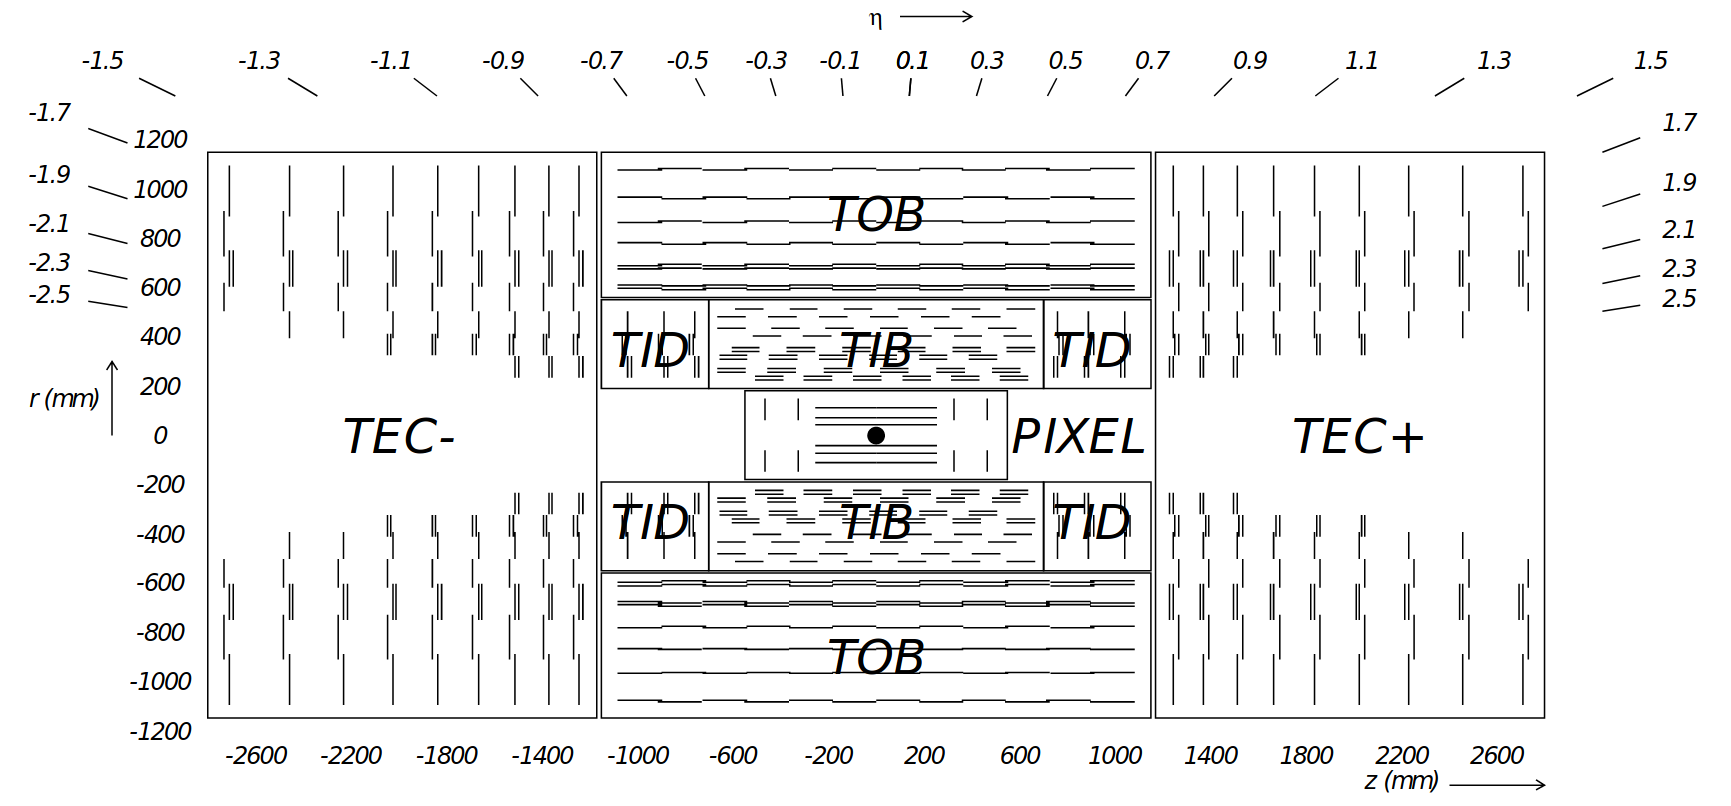
\includegraphics[width=\textwidth]{figures/lhc_and_cms/tracker_layout.png}
\caption{Layout of the CMS silicon tracker. TIB, TOB, TID, and TEC refer to subdetectors of the strip detector while PIXEL refers to the original pixel detector. The Phase-1 pixel detector is contained within the same volume~\cite{cms_experiment}.}
\label{tracker_layout}
\end{figure}

\subsection{Electromagnetic calorimeter}
After traversing the inner tracker, particles next encounter the electromagnetic calorimeter (ECAL). As a homogeneous scintillation calorimeter, ECAL uses \num{61200} lead tungstate crystals in the barrel and \num{7324} in each endcap to reconstruct the energy deposited during electromagnetic showers. Lead tungstate crystals allow for a fast (\SI{80}{\percent} of light emitted within \SI{25}{\ns}), compact (radiation length = \SI{0.89}{cm}), fine-grained (Moli\`ere radius = \SI{2.2}{\cm}), and radiation hard (up to \SI{10}{\mega rad}) calorimeter. The main drawback is the relatively low light yield (\SI{30}{photon\per\mega\electronvolt}), which necessitates photodetectors with intrinsic gain that work in magnetic fields \cite{cms_experiment, cms_tdr_v1}.

The ECAL performance requirements were heavily influenced by the possibility to reconstruct the decay of a Higgs boson to two photons \cite{cms_tdr_v2}. Despite the small branching fraction and irreducible background, this decay channel provides a clean signature of a narrow mass peak on top of a smoothly falling background. Thanks in large part to the excellent ECAL energy resolution, the diphoton channel provided the largest significance and best mass resolution (approximately \SI{1}{\GeV} resolution at \SI{125}{\GeV}) in the CMS Higgs boson discovery in 2012, as shown in Fig.~\ref{higgs_observation_cms} \cite{cms_higgs}.

\begin{figure}[hbtp]
\centering
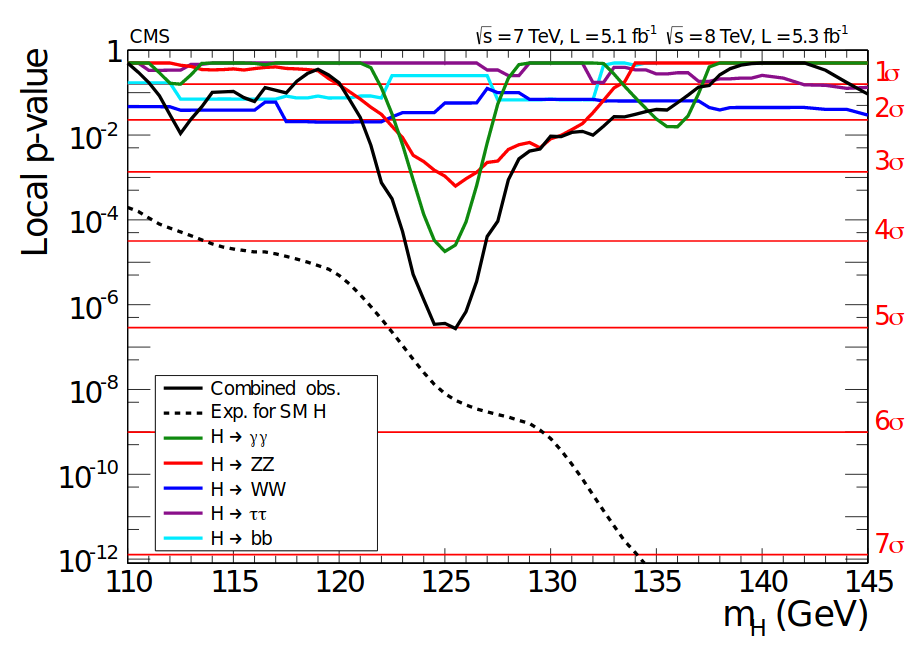
\includegraphics[scale=0.3]{figures/lhc_and_cms/higgs_observation_cms.png}
\caption{The observed local p-value for the five decay modes and the overall combination as a function of the SM Higgs boson mass showing the importance of the ECAL mass resolution in the discovery of the Higgs boson by the CMS experiment. The dashed line shows the expected local p-values for a SM Higgs boson with a mass $m_{H}$ \cite{cms_higgs}.}
\label{higgs_observation_cms}
\end{figure}

The barrel section extends radially from \num{129} to \SI{177}{cm} and covers up to $|\eta|<1.479$. The crystals are tapered to approximately project back to the nominal collision point but not so perfectly that likely particle trajectories align with cracks. Each crystal is approximately one Moli\`ere radius wide and 25 radiation lengths deep. The crystals in each endcap section are arranged in an $x$-$y$ grid that starts at $|z|=\SI{315}{cm}$ and covers $1.479<|\eta|<3.0$.

\fxnote{talk about photodetectors? include picture of crystal and pmt?}

\subsection{Hadronic calorimeter}
Particles that survive the ECAL will next encounter the hadronic calorimeter (HCAL). As the ECAL constitutes approximately 25 radiation lengths but only one interaction length, all but the particles that decay through the strong force will be filtered out before reaching the HCAL. In addition to reconstructing the decays of hadrons, the HCAL plays a particularly important role in measuring \ptmiss. By maximizing the coverage in $\eta$ and overall amount of material in terms of interaction lengths, HCAL ensures that nearly all particles (other than muons, neutrinos, and hypothetical BSM particles) decay and deposit all their energy before reaching the solenoid. Muon momentum is reconstructed with the tracker and muon system, so only neutrinos and hypothetical BSM particles will contribute to \ptmiss. Reliable \ptmiss measurements are particularly important when searching for new weakly interacting particles with large lifetimes such as potential dark matter candidates or R-parity-conserving LSPs\fxnote{cite something?}.

With these goals and the constraint of fitting within the solenoid volume in mind, HCAL is designed as a sampling calorimeter that uses \SI{3.7}{\milli\metre} thick plates of plastic scintillator interspersed within approximately \SI{5}{\cm} thick brass absorber plates to reconstruct the energy deposited during hadronic showers. Embedded wavelength-shifting fibers capture the scintillation light and transfer it to clear fibers to be read out by hybrid photodiodes.\fxnote{why hybrid?}

The barrel section ($|\eta|<1.4$) is segmented into \num{32} towers in $\eta$ and \num{64} in $\phi$ that each contain 17 active scintillator layers. In the $|\eta|<1.26$ range, an extra layer of scintillator tiles (or two at $\eta=0$) sits just outside the solenoid and increases the minimum effective HCAL interaction length to greater than \num{11.8}. Each endcap spans a pseudorapidity range of \num{1.3} to \num{3.0} with \num{14} towers in eta and \num{5} to \SI{10}{\degree} $\phi$ segmentation. Also, a steel and quartz fiber forward calorimeter (HF) sits \SI{11.2}{m} from the interaction point and covers $3<|\eta|<5$. In HF, particles produce Cherenkov light when traversing the quartz fibers that run parallel to the beamline. Figure~\ref{hcal_layout} shows the layout of the barrel, endcap, and forward HCAL subdetectors.
\fxnote{I would prefer more how/why talk and less eta-range talk}

\begin{figure}
\centering
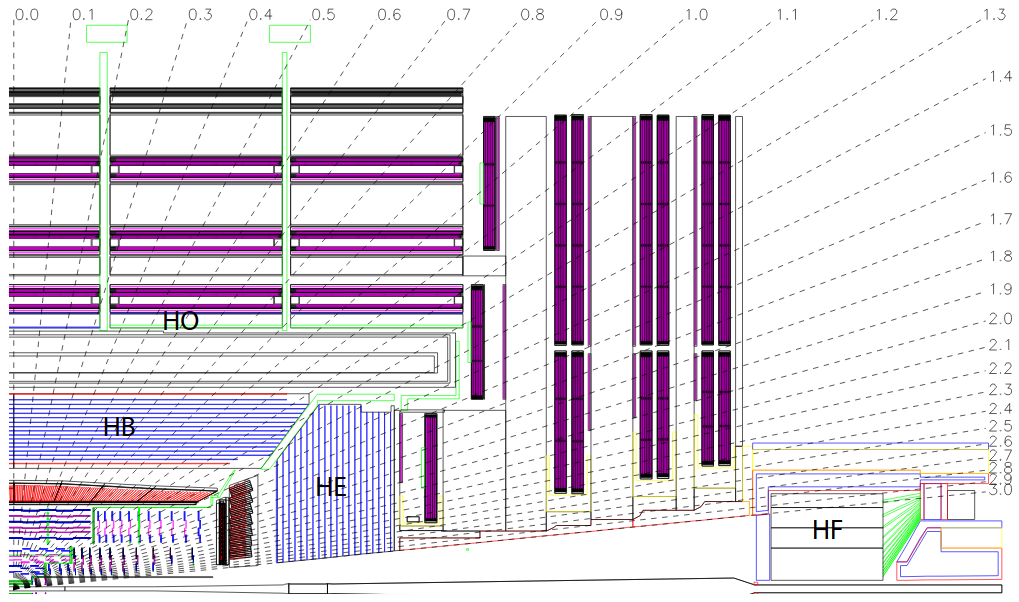
\includegraphics[width=0.8\textwidth]{figures/lhc_and_cms/hcal_layout.png}
\caption{Layout of the hadron calorimeter barrel (HB), outer (HO), endcap (HE), and forward (HF) subdetectors~\cite{cms_experiment}.}
\label{hcal_layout}
\end{figure}

\subsection{Muon system}
The CMS muon system is composed of three varieties of gaseous detectors embedded in the iron return yoke outside the superconducting solenoid. In the central region ($|\eta|<1.2$), the low muon and neutron\fxnote{do I understand neutrons in this context?} rates along with the lower magnetic field allow the use of drift tube (DT) chambers. At higher $\eta$ ($0.9\leq|\eta|<2.4$), cathode strip chambers (CSCs) are required to handle the higher rates and larger magnetic field. Finally, resistive plate chambers (RPCs), which provide more accurate time measurements and worse spatial resolution than the DTs and CSCs, complement the other detectors out to $|\eta|<1.9$ \cite{cms_tdr_v1, cms_ms_performance}.

As shown in Fig.~\ref{muon_momentum_resolution}, the muon momentum resolution of the inner tracker is about an order of magnitude better than that of the muon system for low-\pt muons. The muon system is critical, however, for maintaining the $<10\%$ momentum resolution that is necessary to unambiguously differentiate muons and anti-muons up to \SI{1}{\TeV}. In addition to improving muon reconstruction, the muon system provides information to the L1 trigger (see Section~\ref{trigger}) and is capable of triggering on muons with good efficiency, high background rejection, and about 15--25\% \pt resolution without input from the rest of the detector.

\begin{figure}[hbtp]
\centering
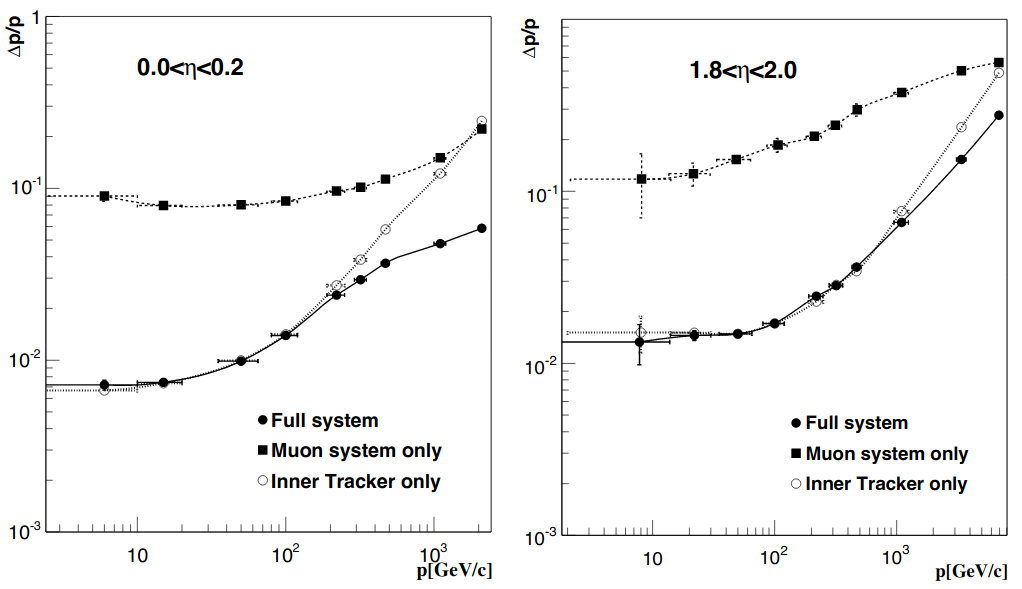
\includegraphics[scale=0.3]{figures/lhc_and_cms/muon_momentum_resolution.png}
\caption{Muon momentum resolution as a function of momentum using the CMS muon system, the CMS inner tracker, and the combination of the two subdetectors in two different $\eta$ ranges \cite{cms_tdr_v1}.}
\label{muon_momentum_resolution}
\end{figure}

The DTs are organized into four stations, each of which contain up to 70 DT chambers that each measure the muon hit position in either the $r$-$\phi$ or $z$ direction. Each chamber is composed of two or three collections of four-layer groupings of \num{13} by \SI{42}{\mm} drift cells. As diagrammed in Fig.~\ref{drift_cell}, a \si{2}--\SI{4}{\m} anode wire runs down the center of each drift cell while electrode and cathode strips line the the top, bottom, and walls of the cell. The cells are filled with an \chem{Ar}/\chem{CO_2} gas mixture that is ionized by charged particles traversing the cell. The liberated electrons cause avalanches in the large electric fields before being collected by the anode wire.

\begin{figure}[hbtp]
\centering
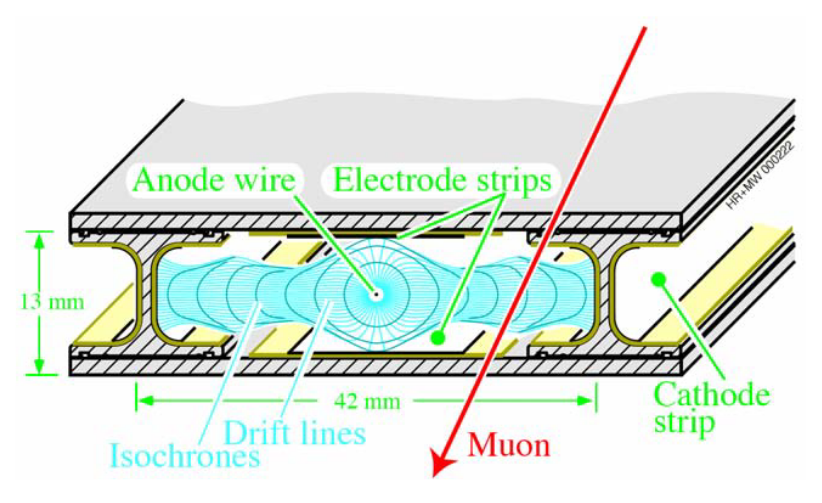
\includegraphics[scale=0.3]{figures/lhc_and_cms/drift_cell}
\caption{Sketch of a CMS muon system drift cell showing drift lines and isochrones.  The plates at the top and bottom of the cell are at ground potential while the voltages applied to the electrodes are +\SI{+3600}{\V} for wires, \SI{+1800}{\V} for strips, and \SI{-1200}{\V} for cathodes \cite{cms_experiment}.}
\label{drift_cell}
\end{figure}

Each endcap contains four CSC stations, each with six layers of CSCs whose cathode strips run radially outward to provide muon hit position measurements in the $r$-$\phi$ plane while the anode wires run in the azimuthal direction to provide measurements in $\eta$. As in the DTs, charged particles ionize a gas mixture inside each chamber (this time an \chem{Ar}/\chem{CO_2}/\chem{CF_4} mixture), which leads to an avalanche of electrons that are collected by an anode wire. In the CSCs, however, several anode wires share the same chamber and a two-coordinate position measurement is obtained by also reading out the induced charge on the perpendicular cathode strips.
\fxnote{add csc or rpc diagrams?}

\fxnote{describe RPCs:
The RPCs are composed of parallel resistive plates separated by two \SI{2}{\mm} gas gaps.}

\subsection{Trigger}
\label{trigger}
The trigger reduces the data writing rate from the \SI{40}{\MHz} collision rate to less than \SI{1}{\kHz} so that events can be written to tape. The rate reduction happens in two stages: Level-1 (L1) and High-Level Trigger (HLT). L1 analyzes input from ECAL, HCAL, and the muon system with custom electronics to reduce the rate to approximately \SI{100}{\kHz} in \SI{3.8}{\us}. With input from all subdetectors, the HLT then uses a dedicated processor farm to further reduce the rate to the desired $<$ 1 kHz \cite{cms_experiment, cms_trigger_upgrade}.
\fxnote{would be nice to expand}

\subsection{Physics object reconstruction}
\label{cms_reco}
CMS uses a particle-flow (PF) algorithm to reconstruct the properties of individual particles from the combination of all subdetector measurements. Starting from charged particle tracks from the tracker and muon system and clusters of energy deposited in the ECAL and HCAL, CMS's PF algorithm aims to reconstruct all final-state electrons, muons, photons, and charged and neutral hadrons in a given event. In this section, I first describe the reconstruction of tracks and energy clusters before moving on to the individual particle identification and reconstruction. A complete description of the CMS PF algorithm is available in Ref.~\cite{cms_pf}.

\subsubsection{Charged particle tracks}
Charged particle tracks are reconstructed with an iterative procedure. Despite the middling reconstruction efficiency of each individual step, starting with the highest-purity algorithms and masking the hits associated with each reconstructed track before moving on to the next step results in higher efficiency than could be achieved with any single tracking algorithm without increasing the rate of misreconstruction.\fxnote{break up this sentence} This general principle applies to all charged particle tracks, but the tracks associated with candidate electrons and muons receive special consideration.

To better handle electron trajectories affected by radiative energy loss, CMS employs a special iterative tracking procedure that includes a Gaussian-sum filter (GSF) \cite{gsf}. This approach improves the overall reconstruction efficiency, allows reconstruction of lower-\pt electrons, and helps identify electrons from photon conversions and distinguish electrons from charged hadrons.

Muon track reconstruction benefits from measurements in the tracker and the muon system. Candidate muon tracks are placed in one of three categories depending on which subdetectors are used in their reconstruction: standalone muon tracks only use muon system hits; tracker muon tracks only use tracker hits and the requirement of at least one consistent muon system hit; and global muon tracks are reconstructed from a global fit of tracker and muon system hits.

\subsubsection{Calorimeter energy clusters}
Energy deposits in the calorimeters are clustered separately in ECAL and HCAL with a Gaussian-mixture model that assumes the energy deposits arise from an arbitrary number of Gaussian energy deposits whose amplitude and location are allowed to vary while the width is determined by the calorimeter properties. The clusters are first seeded by cells with energy above some threshold and greater than the energy of the surrounding cells. Nearby clusters are then merged before being fed to the Gaussian-mixture algorithm. Finally, several corrections are applied to the cluster energies to ensure accurate responses to photons and hadrons.

\subsubsection{Particle-flow reconstruction}
The tracks and clusters are then identified with and used to reconstruct all individual particles in an event. The first step is to link tracks and clusters together into groups that correspond one or a few particles. Tracker tracks are extrapolated outwards and linked with the nearest ECAL and HCAL clusters that are within a set radius in the $\eta$-$\phi$ plane. In the case of candidate electron tracks, tracker tracks and ECAL deposits consistent with electron radiative losses are also linked with the candidate electron track. ECAL and HCAL clusters are similarly linked together by proximity in the $\eta$-$\phi$ plane. Due to the high granularity of CMS subdetectors, the number of tracks and clusters in a linked group is largely independent of the total number of particles in an event.

Each group of linked tracks and clusters is then processed by the PF particle identification and reconstruction algorithm. As in track reconstruction, particle reconstruction is an iterative process in which the tracks and clusters are masked after being associated with a particle. Figure~\ref{cms_slice} diagrams the basic concept used to identify muons, electrons, photons, and charged and neutral hadrons. Each step of the PF algorithm is summarized below.

Muons are reconstructed first from isolated global muon candidates, then non-isolated global muon candidates, and finally tracker muon (standalone muon) candidate tracks that are particularly well measured and consistent with hits in the muon system (tracker). Muon momentum is taken from the tracker track when $\pt<\SI{200}{\GeV}$ and from the combination of tracker and muon system hits that yields the best fit otherwise.

Electron and isolated photon reconstruction, which occur together after muon reconstruction, are necessarily interrelated by the high probability that an electron radiates a photon or a photon pair-produces electrons when interacting with tracker material. Electrons are identified from GSF tracks with a corresponding ECAL cluster while isolated photons are identified from isolated ECAL clusters. The total electron energy accounts for radiative losses that show up as ECAL clusters, and both electrons and isolated photons require a high ratio of ECAL cluster energy to nearby HCAL cluster energy.

Next, nonisolated photons and charged and neutral hadrons are reconstructed from the remaining tracks and clusters. Within the tracker acceptance ($|\eta|<2.5$), ECAL (HCAL) clusters without associated tracks are identified as photons (neutral hadrons). At higher $\eta$, nearby ECAL and HCAL clusters are assumed to arise from the same hadron shower and ECAL clusters without nearby HCAL clusters are identified as photons. Discrepancies between track momenta and associated HCAL cluster energy are also used to identify neutral hadrons and muons. Finally, a post-processing step corrects for rare failure modes that can potentially produce inaccurately large \ptmiss measurements.

\begin{figure}
\centering
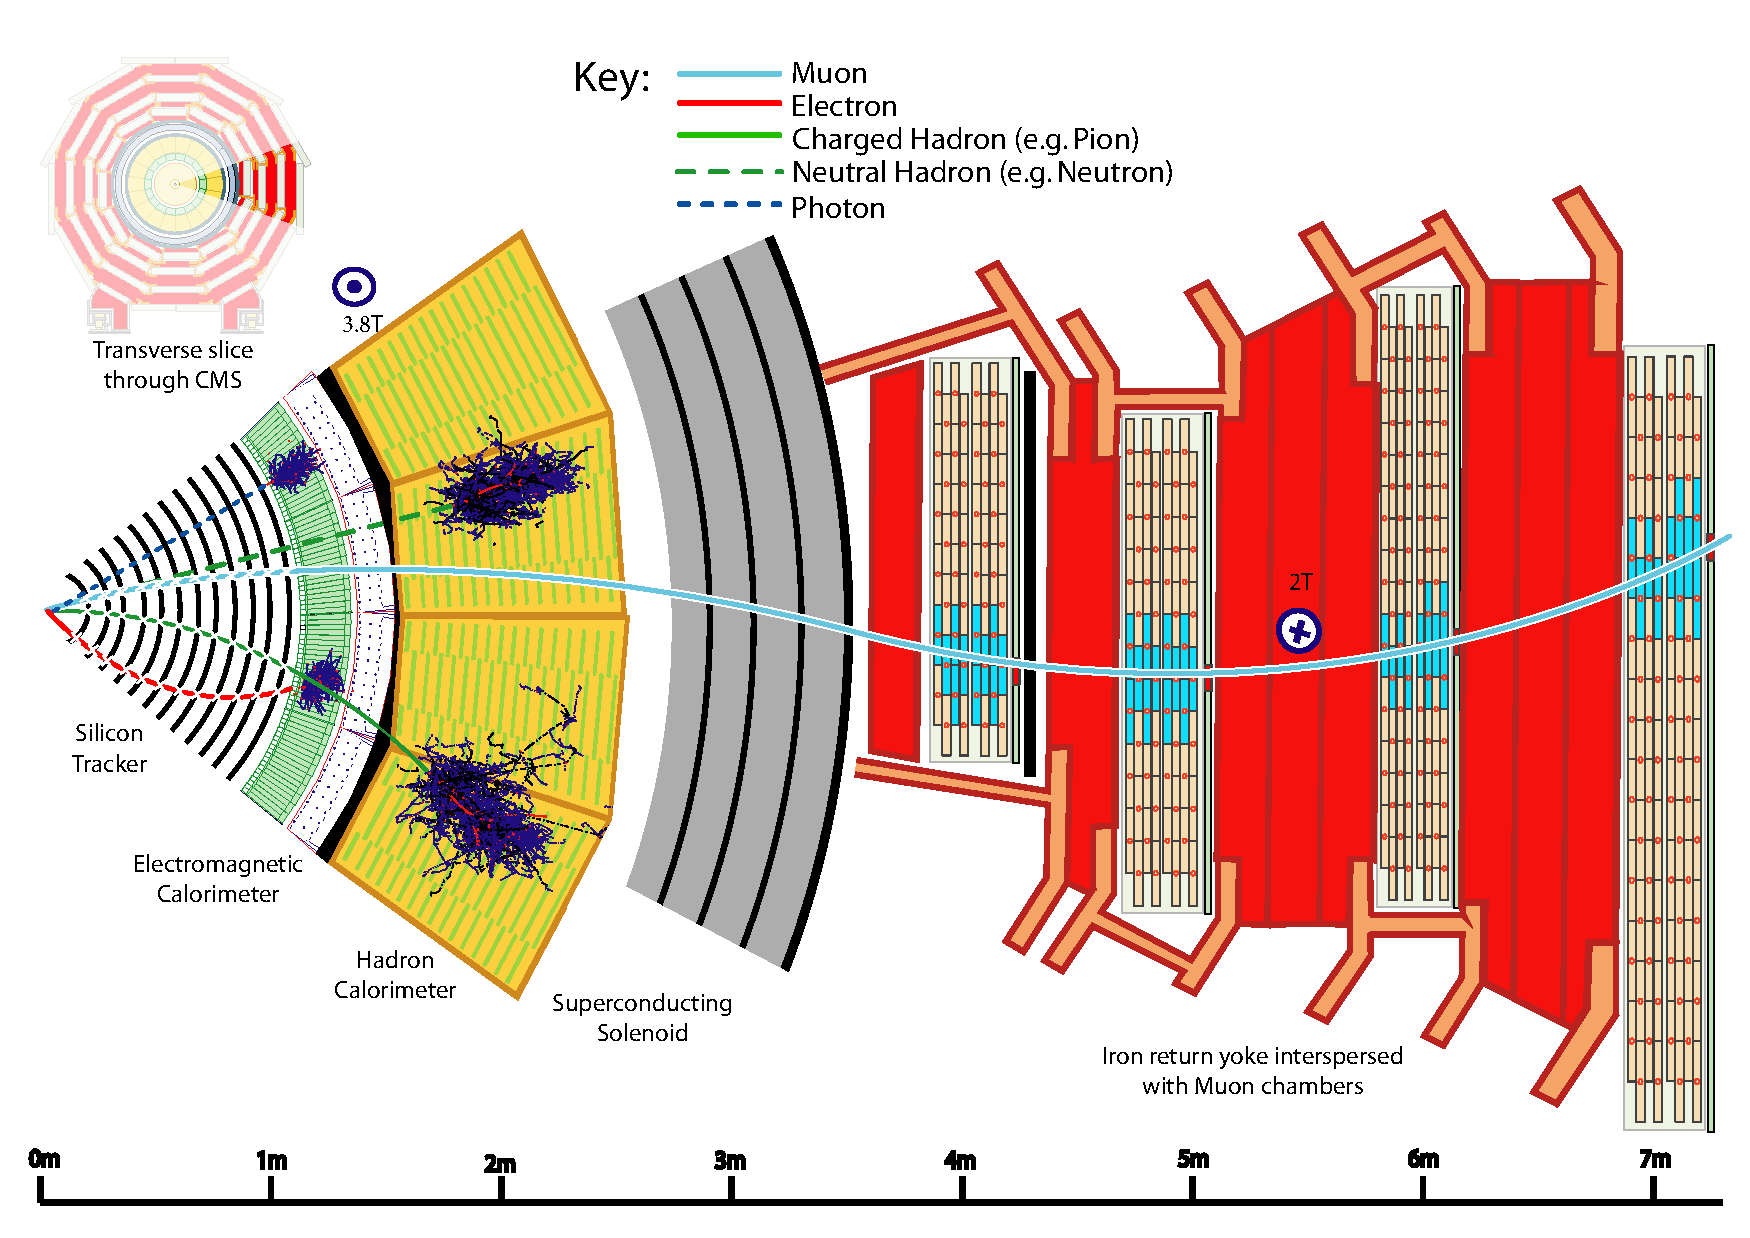
\includegraphics[width=\textwidth]{figures/lhc_and_cms/cms_slice.pdf}
\caption{A sketch of a transverse slice of the CMS detector showing representative particle interactions used to identify and reconstruct particles with the CMS Particle Flow algorithm \cite{cms_pf}.}
\label{cms_slice}
\end{figure}

\pagebreak